\section{Dati e analisi}
Con le impostazioni che ho ricavato nella sezione precedente ho quindi proceduto con la simulazione del comportamento delle onde in presenza di vari potenziali.
\subsection{Il salto di potenziale}
Il primo potenziale che analizzo \`e il salto di potenziale, posiziono un gradino a met\`a del dominio e variandone l'altezza ne calcolo il coefficiente di trasmissivit\`a.

\begin{equation}\label{eq:Salto}
  \lr\{.{\begin{array}{lr}
      V_0& x>a\\
      0&\text{altrove}
  \end{array}}
\end{equation}


Quindi proseguiamo ed eseguiamo delle simulazioni. Per confrontare i risultati delle simulazioni con la teoria ho sostituito in \eqref{eq:riflessioneStepvanilla} $V =  E/x$ notando che il risultato non dipende dall'energia:

\begin{equation}
\lr\{.{\begin{array}{l}
	R =  \frac{2 x -1 -2 \sqrt{x\lrt{x-1}}}{2x -1 +2 \sqrt{x\lrt{x-1}}}\\
	T =  \frac{4 \sqrt{x\lrt{x-1}}}{2x -1 +2 \sqrt{x\lrt{x-1}}}
	\end{array}}
\end{equation}

Nelle simulazioni i lanci sono stati fatti con pacchetti gaussiani inizialmente con $\sigma=0.5$, energia $100$ e massa $10$. Il potenziale \`e stato impostato perch\'e il salto fosse al centro del dominio e con altezza diversa per ogni lancio e ho analizzato l'andamento temporale del rapporto tra l'integrale su tutto il dominio e quello fatto nella prima met\`a.
Ho deciso di usare come coefficiente di riflessione il valore del peso dell'integrale quando questo si \`e stabilizzato.
Dall'andamento nel tempo si pu\`o vedere un piccolo abbassamento quando l'onda impatta il potenziale per le barriere pi\`u alte, prima di venire riflessa all'indietro penetra leggermente nell'area classicamente vietata.

\begin{figure}[htb]
  \centering
  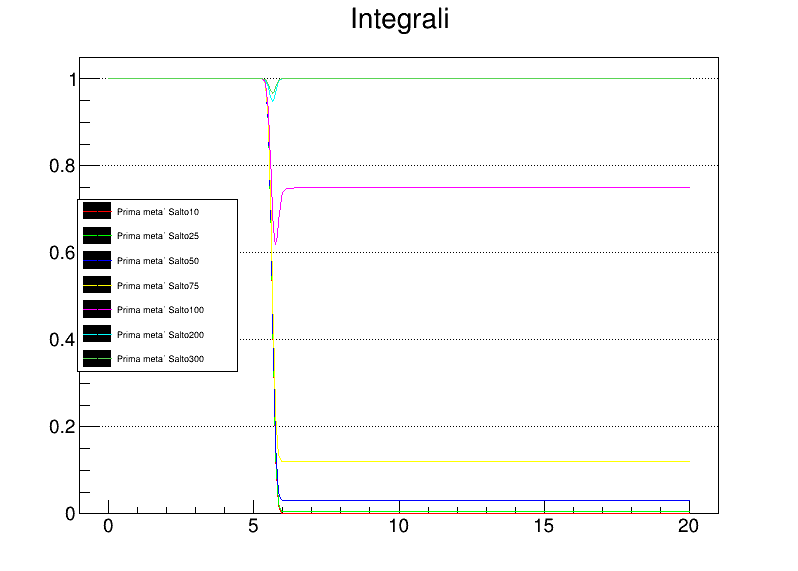
\includegraphics[width=0.7\linewidth]{IMG/SaltoR}
  \caption{I pesi dell'integrale della prima met\`a del dominio per $\sigma=0.5$. Dove c'\`e riflessione si nota una penetrazione parziale dell'onda nella seconda met\`a del dominio seguita dalla riflessione}\label{fig:SaltoR}%RIFARE CON ENERIGA APPROPRIATA
\end{figure}

Come si pu\`o notare dalla \autoref{tab:SaltoDati} sebbene stia simulando un pacchetto d'onda in movimento e non un un'onda piana il peso dei coefficienti ricalca abbastanza bene i coefficienti teorici, e sembra avvicinarli di pi\`u man mano che allargo il pacchetto. Notare che la simulazione si allontana dalla teoria per le onde piane pi\`u si \`e vicini al regime in cui il potenziale \`e maggiore dell'energia dell'onda.

\begin{figure}[hbt]
	\centering
	\begin{subfigure}[b]{0.49\textwidth}
  \begin{tikzpicture}
  \def \En {10};
  \begin{axis}[axis x line = center, axis y line = center, ylabel=R, ylabel style={left}, xlabel=E/V, xlabel style={below right}, xmin = -0.1, xmax = 10.1, ymin=-0.1,ymax =1.1]
  \addplot table[x=ev,y=E\En] {Dati/saltos05.tdt};%{Dati/Salto.tdt};
  \addlegendentry{$\sigma=0.5$}
  	\foreach \sig in {1,2,4}{
  		\addplot table[x=ev,y=E\En] {Dati/saltos\sig.tdt};
  		\edef\temp{\noexpand\addlegendentry{$\sigma = \sig$}}
  		\temp
  	}
  \addplot[domain=0:10, samples =501, green]	plot[id=Refl2]	function{\Rjump(x)};
  \addlegendentry{teoria}
  \end{axis}
  \end{tikzpicture}
	\end{subfigure}
	~
	\begin{subfigure}[b]{0.49\textwidth}
  \begin{tikzpicture}
  \def \sig {2};
  \begin{axis}[axis x line = center, axis y line = center, ylabel=R, ylabel style={left}, xlabel=E/V, xlabel style={below right}, xmin = -0.1, xmax = 10.1, ymin=-0.1,ymax =1.1]
  	\foreach \E in {10,15,20,25}{
		\addplot table[x=ev,y=E\E] {Dati/saltos\sig.tdt};
		\edef\temp{\noexpand\addlegendentry{$E=\E$}}
		\temp
	}
  \addplot[domain=0:10, samples =501, green]	plot[id=Refl2]	function{\Rjump(x)};
  \addlegendentry{teoria}
  \end{axis}
  \end{tikzpicture}
	\end{subfigure}
  \caption{La visualizzazione dei dati e il confronto con la teoria, il primo grafico fatto con $E=10$, il secondo con $\sigma = 2$}
\end{figure}

Dai grafici si nota che se $\sigma$ \`e piccolo c'\`e una tendenza  a deviare dal comportamento teorico, mentre variando l'energia non sembrano esserci differenze

%%%%%%%%%%%%%%%%%%%%%%%%%%%%%%%%%%%%%%%%%%%%%%%%%%%%%%%%%%%%%%%%%%%%%%%%%%%%%%%%%%%%%%%%%%%%%%%%%
%%%%%%%%%%%%%%%%%%%%%%%%%%%%%%%%%%%%%%%%%%%%%%%%%%%%%%%%%%%%%%%%%%%%%%%%%%%%%%%%%%%%%%%%%%%%%%%%%
%%%%%%%%%%%%%%%%%%%%%%%%%%%%%%%%%%%%%%%%%%%%%%%%%%%%%%%%%%%%%%%%%%%%%%%%%%%%%%%%%%%%%%%%%%%%%%%%%
%%%%%%%%%%%%%%%%%%%%%%%%%%%%%%%%%%%%%%%%%%%%%%%%%%%%%%%%%%%%%%%%%%%%%%%%%%%%%%%%%%%%%%%%%%%%%%%%%
\subsection{La barriera rettangolare}
Ho quindi simulato il comportamento dell'onda in presenza di una barriera rettangolare:

\begin{equation}\label{eq:Barriera}
  \lr\{.{\begin{array}{lr}
      V_0& 0<x<a\\
      0&\text{altrove}
  \end{array}}
\end{equation}

Ho svolto la teoria nella \autoref{sec:BarrieraCalc}.
I grafici che in seguito riporter\`o mostrano il valore del modulo della forma d'onda contenuta nella parte di dominio a sinistra della barriera che corrisponde al coefficiente di riflessione della teoria per le onde piane. I grafici sono disegnati in funzione del rapporto $ E/V$, dato che nelle simulazioni ho variato il valore del potenziale ho sostituito $V = E/x$ in \eqref{eq:riflessionevanilla} per poterla visualizzare come confronto teorico:

\begin{equation}
R\lrt{m,E,x} = \lr\{.{\begin{array}{lr}
	\lrt{1+4 \frac{\lrt{x-x^2}}{\sinh^2\lrt{a \sqrt{2m E\lrt{1/x-1}}}}}^{-1} & 0<x<1 \\
	\lrt{1+\frac{2}{ a^2 m E}}^{-1}                                             & x=1 \\
	\lrt{1+4 \frac{\lrt{x^2 - x}}{\sin^2\lrt{a \sqrt{2m E\lrt{1-1/x}}}}}^{-1} & x>1
	\end{array}}
\end{equation}

%\begin{figure}[hbt]
%	\centering
%	\begin{tikzpicture}
%	\begin{axis}[axis x line = center, axis y line = center, ylabel=R, ylabel style={left}, xlabel=E/V, xlabel style={below right}, xmin = -0.1, xmax = 3.1, ymin=-0.1,ymax =1.1]
%	\foreach \a/\En/\mycol in {2/10/red,2/15/blue,4/10/green,4/15/orange}{
%		\addplot[domain=0.1:4, samples =501, \mycol]	gnuplot	{\Rbarrier(x,10,\En,\a)};
%		\edef\temp{\noexpand\addlegendentry{$a=\a$, $E=\En$}}
%		\temp
%	}
%%	\def \a {2}
%%	\def \En{10}
%%	\addplot[domain=0.1:4, samples =501, red]	gnuplot	{\Rbarrier(x,10,\En,\a)};
%%	\addlegendentry{$a=\a$, $E=\En$}
%%	\def \En{15}
%%	\addplot[domain=0.1:4, samples =501, blue]	gnuplot	{\Rbarrier(x,10,\En,\a)};
%%	\addlegendentry{$a=\a$, $E=\En$}
%%	\def \a {4}
%%	\def \En{10}
%%	\addplot[domain=0.1:4, samples =501, green]	gnuplot	{\Rbarrier(x,10,\En,\a)};
%%	\addlegendentry{$a=\a$, $E=\En$}
%%	\def \En{15}
%%	\addplot[domain=0.1:4, samples =501, orange]	gnuplot	{\Rbarrier(x,10,\En,\a)};
%%	\addlegendentry{$a=\a$, $E=\En$}
%	\end{axis}
%	\end{tikzpicture}
%	\caption{La teoria per alcuni valori di $E$ e di $a$, tenendo fissa la massa a $m=5$}
%\end{figure}

\begin{figure}[hbt]
  \centering
  \begin{tikzpicture}
    \def \a {2}
    \begin{axis}[axis x line = center, axis y line = center, ylabel=R, ylabel style={left}, xlabel=E/V, xlabel style={below right}, xmin = -0.1, xmax = 10.1, ymin=-0.1,ymax =1.1]
      \foreach \sig in {0.5,1,2,4}{
      	\addplot table[x=ev,y=s\sig] {Dati/Barriera_a1.tdt};
      	\edef\temp{\noexpand\addlegendentry{$\sigma = \sig$}}
      	\temp
      }
      \addplot[domain=0.1:10, samples =501, red]	gnuplot	{\Rbarrier(x,10,5,1)};
      \addlegendentry{teoria $a=2$ }
    \end{axis}
  \end{tikzpicture}
  \caption{La visualizzazione dei dati e il confronto con la teoria, con $E=5$, $m=10$ e $a=1$}\label{fig:Barriera}
\end{figure}

\begin{figure}[hbt]
  \centering
  \begin{subfigure}[b]{0.49\textwidth}
    \begin{tikzpicture}
      \begin{axis}[axis x line = center, axis y line = center, ylabel=R, ylabel style={left}, xlabel=E/V, xlabel style={below right}, xmin = 1.9, xmax = 4.1, ymin=-0.001,ymax = 0.11]
\foreach \sig in {0.5,1,2,3}{
	\addplot table[x=ev,y=s\sig] {Dati/DataOsc2.tdt};
	\edef\temp{\noexpand\addlegendentry{$a=2$, $\sigma=\sig$}}
	\temp
}
      \def \a {2};
      \def \m {10};
      \def \En {15};
	\addplot[domain=2:4, samples =501, blue]	plot[id=MRefl2z]	function{\Rbarrier (x,\m,\En,\a)};
	\addlegendentry{teoria a=\a}
	\addplot[domain=2:4, samples =501, red]	plot[id=Refl2]	function{\Rjump (x)};
	\addlegendentry{teoria scalino}
      \end{axis}
    \end{tikzpicture}
  \end{subfigure}
  ~
  \begin{subfigure}[b]{0.49\textwidth}
    \begin{tikzpicture}
      \def \a {2}
      \begin{axis}[axis x line = center, axis y line = center, ylabel=R, ylabel style={left}, xlabel=E/V, xlabel style={below right}, xmin = 1.9, xmax = 4.1, ymin=-0.001,ymax = 0.11]
	\foreach \sig in {4,5,6,7}{
		\addplot table[x=ev,y=s\sig] {Dati/DataOsc2.tdt};
		\edef\temp{\noexpand\addlegendentry{$a=2$, $\sigma=\sig$}}
	  \temp
	}
      \def \a {2};
      \def \m {10};
      \def \En {15};
      \addplot[domain=2:4, samples =501, blue]	plot[id=MRefl2z]	function{\Rbarrier (x,\m,\En,\a)};
      \addlegendentry{teoria a=\a}
	\addlegendentry{teoria a=\a}
      \end{axis}
    \end{tikzpicture}
  \end{subfigure}
  \caption{I dati tra 2 e 4 per una barriera larga 2, con $E=15$}\label{fig:Osc2}
\end{figure}


\begin{figure}[hbt]
  \centering
  \begin{subfigure}[b]{0.49\textwidth}
    \begin{tikzpicture}
      \def \a {4}
      \begin{axis}[axis x line = center, axis y line = center, ylabel=R, ylabel style={left}, xlabel=E/V, xlabel style={below right}, xmin = 1.9, xmax = 4.1, ymin=-0.001,ymax = 0.11]
            \foreach \sig in {0.5,1,2,3}{
            	\addplot table[x=ev,y=s\sig] {Dati/data.tdt};
            	\edef\temp{\noexpand\addlegendentry{$a=2$, $\sigma=\sig$}}
            	\temp
            }
      \def \a {4};
      \def \m {10};
      \def \En {15};
      \addplot[domain=2:4, samples =501, blue]	plot[id=MRefl2z]	function{\Rbarrier (x,\m,\En,\a)};
      \addlegendentry{teoria a=\a}
	\addplot[domain=2:4, samples =501, red]	plot[id=Refl2]	function{\Rjump (x)};
	\addlegendentry{teoria scalino}
      \end{axis}
    \end{tikzpicture}
  \end{subfigure}
  ~
  \begin{subfigure}[b]{0.49\textwidth}
    \begin{tikzpicture}
      \def \a {8}
      \begin{axis}[axis x line = center, axis y line = center, ylabel=R, ylabel style={left}, xlabel=E/V, xlabel style={below right}, xmin = 1.9, xmax = 4.1, ymin=-0.001,ymax = 0.11]
            \foreach \sig in {4,5,6,7}{
            	\addplot table[x=ev,y=s\sig] {Dati/data.tdt};
            	\edef\temp{\noexpand\addlegendentry{$a=2$, $\sigma=\sig$}}
            	\temp
            }
      \def \a {4};
      \def \m {10};
      \def \En {15};
      \addplot[domain=2:4, samples =501, blue]	plot[id=MRefl2z]	function{\Rbarrier (x,\m,\En,\a)};
      \addlegendentry{teoria a=\a}
      \end{axis}
    \end{tikzpicture}
  \end{subfigure}
  \caption{I dati tra 2 e 4 per una barriera larga 4, con $E=15$}\label{fig:Osc4}
\end{figure}

Voglio provare a replicare le oscillazioni che si notano in \autoref{fig:Barriera}.
Faccio simulazioni pi\`u ''fitte`` in un intervallo del rapporto di $E/V$ p\`u piccolo e con $E=15$.
La prima cosa che si pu\`o osservare dai dati \`e che pi\`u la barriera \`e  grande rispetto alla larghezza del pacchetto pi\`u la simulazione si allontana dalla teoria per le onde piane.
Probabilmente questo \`e dovuto al fatto che se il pacchetto incontra una barriera pi\`u ''larga`` delle sue dimensioni questo tenda a comportarsi similmente a come se fosse in presenza di un salto di potenziale ma da \autoref{fig:Osc2} e \autoref{fig:Osc4} si nota che questa mia idea non \`e del tutto corretta: l'andamento \`e simile ma la barriera riflette di p\`u rispetto al salto singolo questo probabilmente \`e dovuto al fatto che  anche quando un potenziale cala si presentano riflessioni e questo contribuisce a far crescere il coefficiente di riflessione.


\begin{figure}[hbt]
  \centering
  \begin{subfigure}[b]{0.49\textwidth}
    \begin{tikzpicture}
      \def \a {0.1};
      \def \m {5};
      
      \begin{axis}[axis x line = center, axis y line = center, ylabel=R, ylabel style={left}, xlabel=E/V, xlabel style={below right}, xmin = 0.25, xmax = 1.75, ymin=-0.1,ymax =1.1]
	\def \En {25};
	\addplot table[x=ev,y=E25] {Dati/datatunnelm5.tdt};
	\addlegendentry{S: $E=25$}
	\addplot[domain=0.25:1.75, samples =501, orange]	plot[id=MTunnel525]	function{(\Rbarrier (x,\m,\En,\a)};
	\addlegendentry{T: $E=25$}
	\def \En {75};
	\addplot table[x=ev,y=E75] {Dati/datatunnelm5.tdt};
	\addlegendentry{S: $E=75$}
	\addplot[domain=0.25:1.75, samples =501, green]	plot[id=MTunnel575]	function{\Rbarrier (x,\m,\En,\a)};
	\addlegendentry{T: $E=75$}
      \end{axis}
    \end{tikzpicture}
  \end{subfigure}
  ~
  \begin{subfigure}[b]{0.49\textwidth}
    \begin{tikzpicture}
      \def \a {0.1};
      \def \m {5};
      
      \begin{axis}[axis x line = center, axis y line = center, ylabel=R, ylabel style={left}, xlabel=E/V, xlabel style={below right}, xmin = 0.25, xmax = 1.75, ymin=-0.1,ymax =1.1]
	\def \En {50};
	\addplot table[x=ev,y=E50] {Dati/datatunnelm5.tdt};
	\addlegendentry{S: $E=50$}
	\addplot[domain=0.25:1.75, samples =501, orange]	plot[id=MTunnel550]	function{\Rbarrier (x,\m,\En,\a)};
	\addlegendentry{T: $E=50$}
	\def \En {100};
	\addplot table[x=ev,y=E100] {Dati/datatunnelm5.tdt};
	\addlegendentry{S: $E=100$}
	\addplot[domain=0.25:1.75, samples =501, green]	plot[id=MTunnel5100]	function{\Rbarrier (x,\m,\En,\a)};
	\addlegendentry{T: $E=100$}
      \end{axis}
    \end{tikzpicture}
  \end{subfigure}
  \caption{Provo a simulare l'effetto tunnel, impiegando un pacchetto con $\sigma = 4$, con massa delle particelle 5 e spessore della barriera $a=0.1$}
\end{figure}

\begin{figure}[hbt]
  \centering
  \begin{subfigure}[b]{0.49\textwidth}
    \begin{tikzpicture}
      \def \a {0.1};
      \def \m {10};
      
      \begin{axis}[axis x line = center, axis y line = center, ylabel=R, ylabel style={left}, xlabel=E/V, xlabel style={below right}, xmin = 0.25, xmax = 1.75, ymin=-0.1,ymax =1.1]
	\def \En {25};
	\addplot table[x=ev,y=E25] {Dati/datatunnelm10.tdt};
	\addlegendentry{S: $E=25$}
	\addplot[domain=0.25:1.75, samples =501, orange]	plot[id=MTunnel525]	function{\Rbarrier (x,\m,\En,\a)};
	\addlegendentry{T: $E=25$}
	\def \En {75};
	\addplot table[x=ev,y=E75] {Dati/datatunnelm10.tdt};
	\addlegendentry{S: $E=75$}
	\addplot[domain=0.25:1.75, samples =501, green]	plot[id=MTunnel575]	function{\Rbarrier (x,\m,\En,\a)};
	\addlegendentry{T: $E=75$}
      \end{axis}
    \end{tikzpicture}
  \end{subfigure}
  ~
  \begin{subfigure}[b]{0.49\textwidth}
    \begin{tikzpicture}
      \def \a {0.1};
      \def \m {10};
      
      \begin{axis}[axis x line = center, axis y line = center, ylabel=R, ylabel style={left}, xlabel=E/V, xlabel style={below right}, xmin = 0.25, xmax = 1.75, ymin=-0.1,ymax =1.1]
	\def \En {50};
	\addplot table[x=ev,y=E50] {Dati/datatunnelm10.tdt};
	\addlegendentry{S: $E=50$}
	\addplot[domain=0.25:1.75, samples =501, orange]	plot[id=MTunnel550]	function{\Rbarrier (x,\m,\En,\a)};
	\addlegendentry{T: $E=50$}
	\def \En {100};
	\addplot table[x=ev,y=E100] {Dati/datatunnelm10.tdt};
	\addlegendentry{S: $E=100$}
	\addplot[domain=0.25:1.75, samples =501, green]	plot[id=MTunnel5100]	function{\Rbarrier (x,\m,\En,\a)};
	\addlegendentry{T: $E=100$}
      \end{axis}
    \end{tikzpicture}
  \end{subfigure}
  \caption{Provo a simulare l'effetto tunnel, impiegando un pacchetto con $\sigma = 4$, con massa delle particelle 10 e spessore della barriera $a=0.1$}
\end{figure}

\begin{figure}[hbt]
  \centering
  \begin{subfigure}[b]{0.49\textwidth}
    \begin{tikzpicture}
      \def \a {0.1};
      \def \m {15};
      
      \begin{axis}[axis x line = center, axis y line = center, ylabel=R, ylabel style={left}, xlabel=E/V, xlabel style={below right}, xmin = 0.25, xmax = 1.75, ymin=-0.1,ymax =1.1]
	\def \En {25};
	\addplot table[x=ev,y=E25] {Dati/datatunnelm15.tdt};
	\addlegendentry{S: $E=25$}
	\addplot[domain=0.25:1.75, samples =501, orange]	plot[id=MTunnel525]	function{(x==1)?1-2/(2+\a*\a*\En*\m):1+(8*(x-1)*x)/(cos(2*\a*sqrt(2*\m*\En*(x-1)))-1-8*x*(x-1))};
	\addlegendentry{T: $E=25$}
	\addplot table[x=ev,y=E75] {Dati/datatunnelm15.tdt};
	\addlegendentry{S: $E=75$}
	\def \En {75};
	\addplot[domain=0.25:1.75, samples =501, green]	plot[id=MTunnel575]	function{(x==1)?1-2/(2+\a*\a*\En*\m):1+(8*(x-1)*x)/(cos(2*\a*sqrt(2*\m*\En*(x-1)))-1-8*x*(x-1))};
	\addlegendentry{T: $E=75$}
      \end{axis}
    \end{tikzpicture}
  \end{subfigure}
  ~
  \begin{subfigure}[b]{0.49\textwidth}
    \begin{tikzpicture}
      \def \a {0.1};
      \def \m {15};
      
      \begin{axis}[axis x line = center, axis y line = center, ylabel=R, ylabel style={left}, xlabel=E/V, xlabel style={below right}, xmin = 0.25, xmax = 1.75, ymin=-0.1,ymax =1.1]
	\def \En {50};
	\addplot table[x=ev,y=E50] {Dati/datatunnelm15.tdt};
	\addlegendentry{S: $E=50$}
	\addplot[domain=0.25:1.75, samples =501, orange]	plot[id=MTunnel550]	function{(x==1)?1-2/(2+\a*\a*\En*\m):1+(8*(x-1)*x)/(cos(2*\a*sqrt(2*\m*\En*(x-1)))-1-8*x*(x-1))};
	\addlegendentry{T: $E=50$}
	\def \En {100};
	\addplot table[x=ev,y=E100] {Dati/datatunnelm15.tdt};
	\addlegendentry{S: $E=100$}
	\addplot[domain=0.25:1.75, samples =501, green]	plot[id=MTunnel5100]	function{(x==1)?1-2/(2+\a*\a*\En*\m):1+(8*(x-1)*x)/(cos(2*\a*sqrt(2*\m*\En*(x-1)))-1-8*x*(x-1))};
	\addlegendentry{T: $E=100$}
      \end{axis}
    \end{tikzpicture}
  \end{subfigure}
  \caption{Provo a simulare l'effetto tunnel, impiegando un pacchetto con $\sigma = 4$, con massa delle particelle 15 e spessore della barriera $a=0.1$}
\end{figure}

A questo punto provo a diminuire le dimensioni della barriera per provare l'effetto tunnel: guardo quanto cala il coefficiente di riflessione quando il rapporto tra $E/V$ \`e inferiore a 1. Vario la massa del pacchetto
%in \autoref{fig:TunnelM}
e le dimensioni della barriera
%in \autoref{fig:TunnelDim}